This chapter will analyse how accurate the IPS is and will critically analyse the delivered solution. The requirements from chapter 3 will provide the basis for the functional evaluation of the project. In addition, the project will be evaluated from a non-functional perspective. The section \ref{sec:comparison} will provide a comparison between the existing solutions and the solution developed by our project.

\section{IPS Performance and Accuracy Analysis}
\label{sec:accuracy}

The majority of the data was collected from the South Wing of Bush House in this project, as the North Wing houses the academic offices, with restricted access. The data collection started using only one computer lab, and progressively the data set was extended to the corridor, to surrounding computer labs, and across the other floors of the Informatics Department. It has been assumed that if the algorithm performs well on a small and restricted data set, such as one or two rooms, which are very close to each other, on a larger scale, the performance should stay the same, if not improve. Only one wing of Bush House has been mainly used for testing, because on the other wing, the academic offices are found, and the area is slightly restricted. 

To evaluate the IPS, the data was collected using the admin application on an iPad. It is strongly recommended that data collection is done on a tablet due to the higher amount of precision when inputting locations onto the floor plan.

The positioning algorithm has been tested in different scenarios. First, given a data set, the goal of the tests were to position the user as accurately as possible in a room where the measurements are known. Measurements have been recorded having approximately 2m between themselves. However, certain positions in a room have been inaccessible due to the position of the chairs or tables. Taking this into account, the algorithm places the user in the location that matches the data set the best, therefore, the accuracy of the algorithm is $\approx 2$ meters. The results given this configuration can be seen in figure 6.1. 

\begin{figure}[H]
    \centering
    \fbox{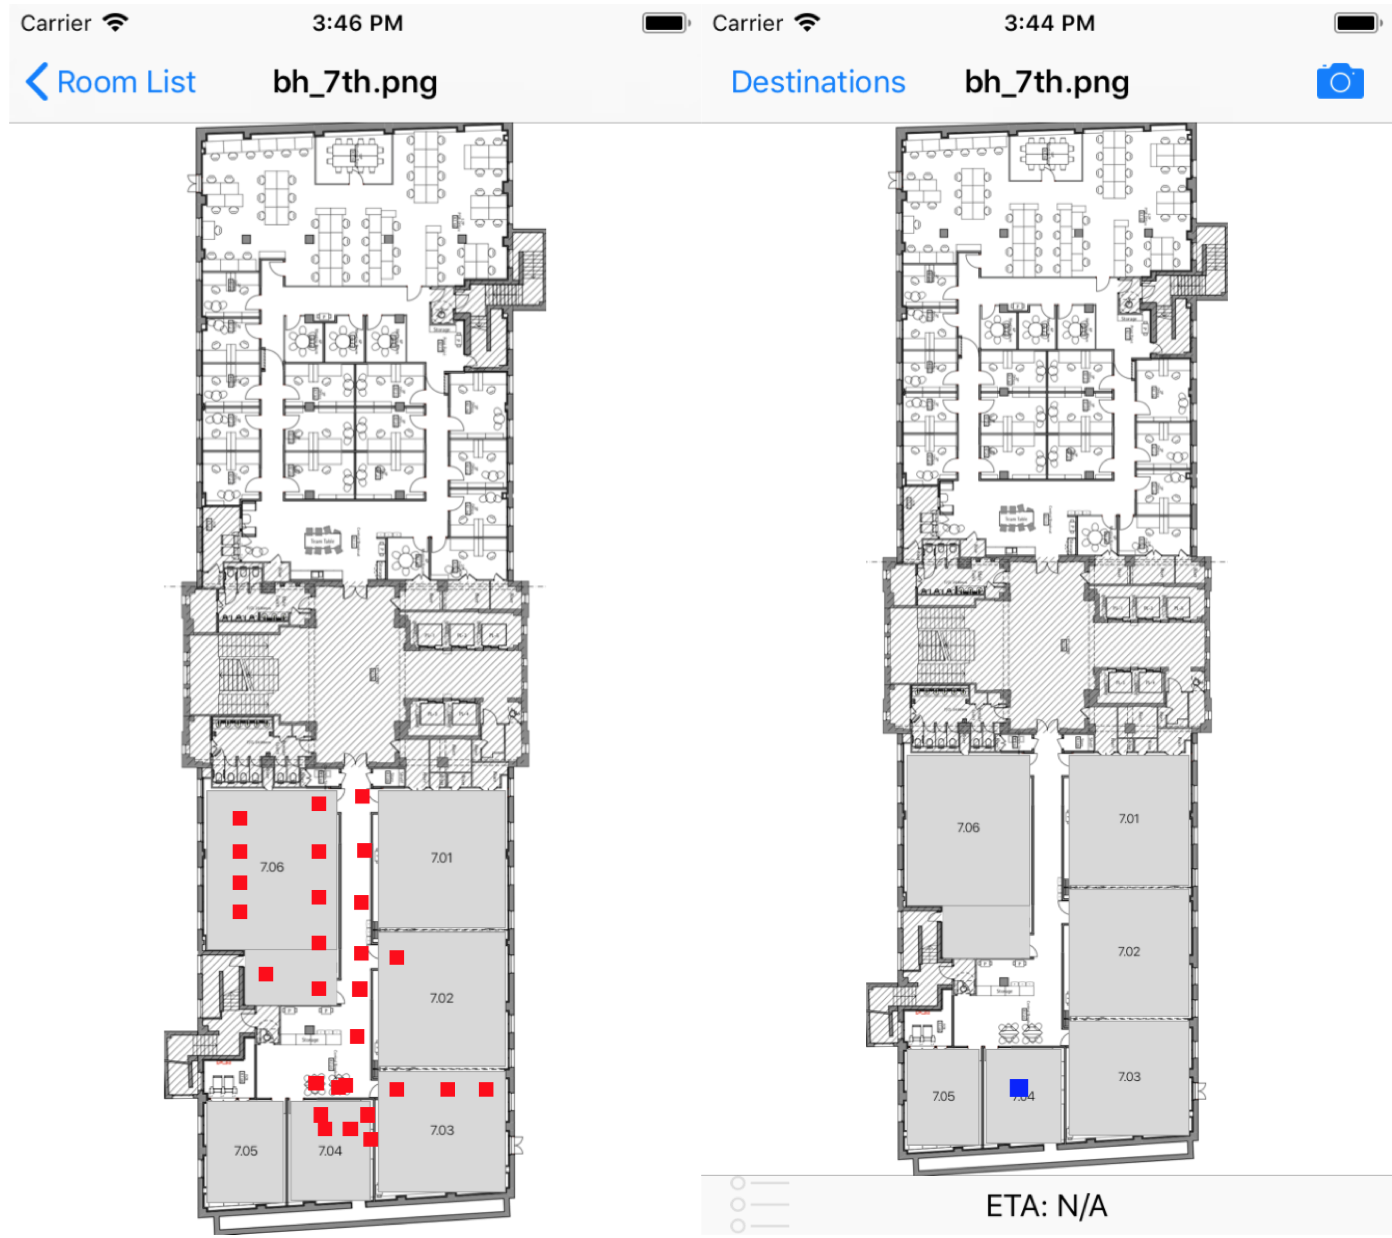
\includegraphics[width=300px, height=268px]{Evaluation/known-loc.png}}
    \caption{Positioning with known locations. The squares in red represent the recorded locations and the square in blue represents the position determined by the algorithm. The screen shot on the left is from the admin application, and the screen shot on the right is from the user application.}
    \label{fig:ips-known-loc}
\end{figure}

\newpage
The second scenario the algorithm has been tested in was when data has not been measured for a room previously, to see how the algorithm behaves when there is no data available. In this case, based on the Wi-Fi networks that are around, the algorithm find the closest recorded position (see fig \ref{fig:ips-unknown-loc}.

\begin{figure}[H]
    \centering
    \fbox{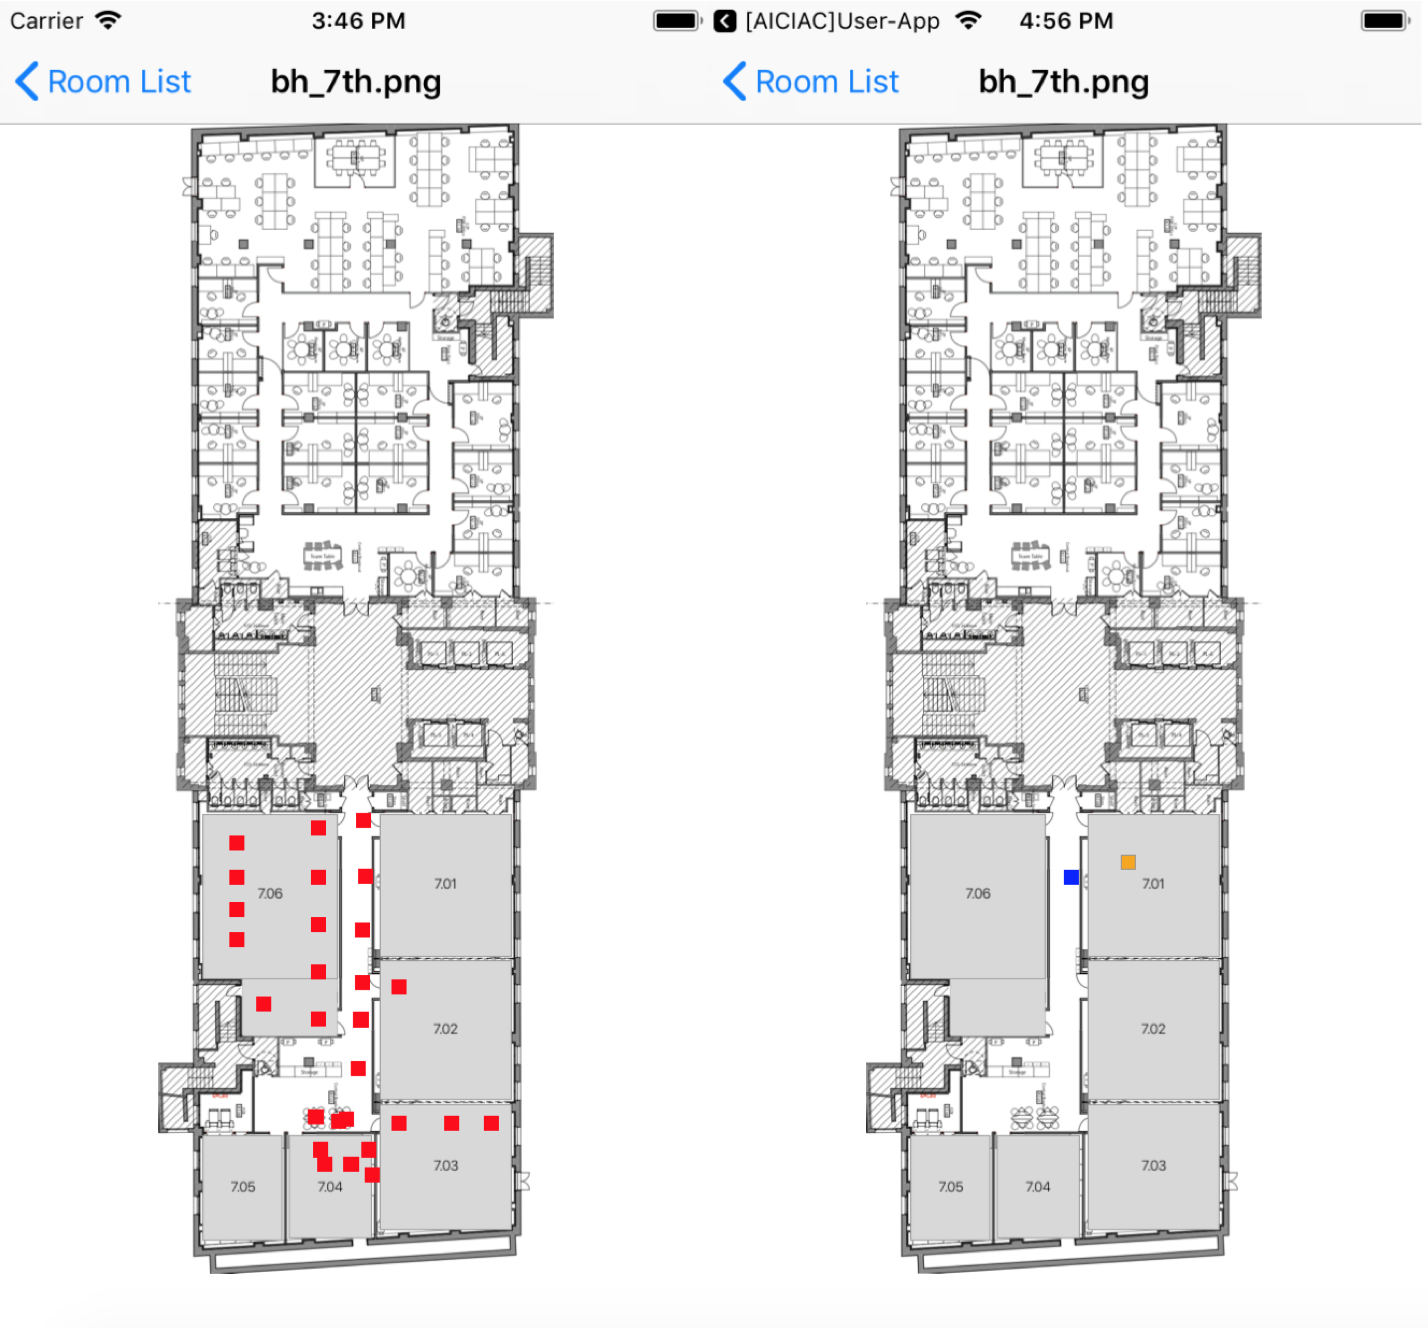
\includegraphics[width=300px, height=279px]{Evaluation/unknown-loc.png}}
    \caption{Positioning with unknown locations. The squares in red represent the recorded locations. The floor plan on the right shows where the algorithm has found the closest location (blue) compared to the current position (orange).}
    \label{fig:ips-unknown-loc}
\end{figure}

\section{Path Finding Algorithm Analysis}
\label{sec:nav-analysis}
The testing approach for the IPS algorithm was also adopted to test the path finding algorithm. The algorithm was tested first with locations in the same room, then between two adjacent rooms, and finally from wing to wing. To test the algorithm, convenient positions have been recorded in order for the path to be shown in a user friendly way on the floor plan (e.g. in front of doors; in this way the path will line up perfectly on the screen and they will not be placed on top of walls). One of the large scale tests was conducted from the end of the South Wing to Dr. Cole's office. Figure \ref{fig:nav-long-path} shows an example where the algorithm has been successful in finding a path between the two locations.

\begin{figure}[H]
    \centering
    \fbox{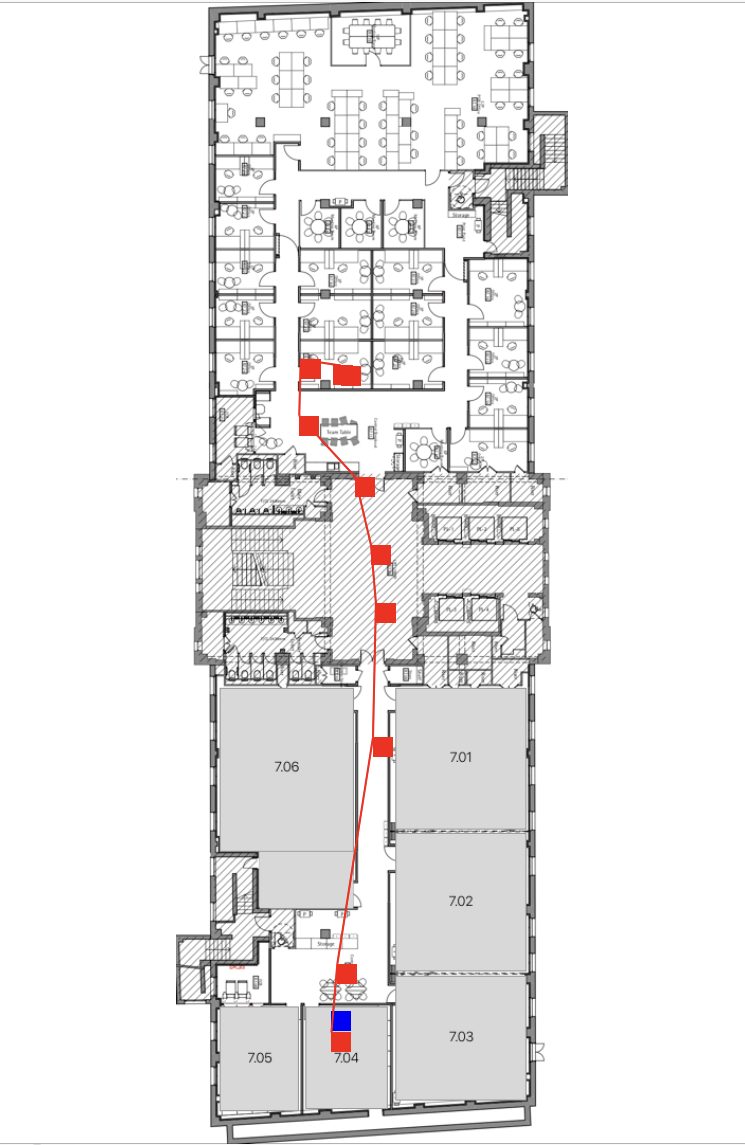
\includegraphics[width=180px, height=280px]{Evaluation/long-path.png}}
    \caption{Long path between a computer lab in the South Wing and Dr Cole's office on the North Wing of Bush House. The square in blue represents the current position of the user and the squares in red represent the way-points to follow. The last red square represents the destination.}
    \label{fig:nav-long-path}
\end{figure}

\section{AR Features Results}
\label{sec:ar-results}
Another fundamental aim of this project was to implement AR features. In combination with the path finding algorithm, the first AR feature facilitates the navigation process by showing the direction the user should follow, based on the smart-phone's built-in compass. The user mobile app shows the proposed visual cue, however during multiple tests, the bearing angle of the visual cue proved to be inaccurate. The magnetic field created by the multitude of radio frequencies from the Wi-Fi networks, together with the magnetic field produced by the Raspberry Pi, which needs to be in the proximity of the smart-phone are causing reflections which impact the bearing angle. However, moving around reduces the effect of the reflections, because this allows time for the compass to calibrate. Figure \ref{fig:ar-arrow} shows a screen shot of the user app which includes the AR navigation guidance to direct the user to their final destination.

\begin{figure}[H]
    \centering
    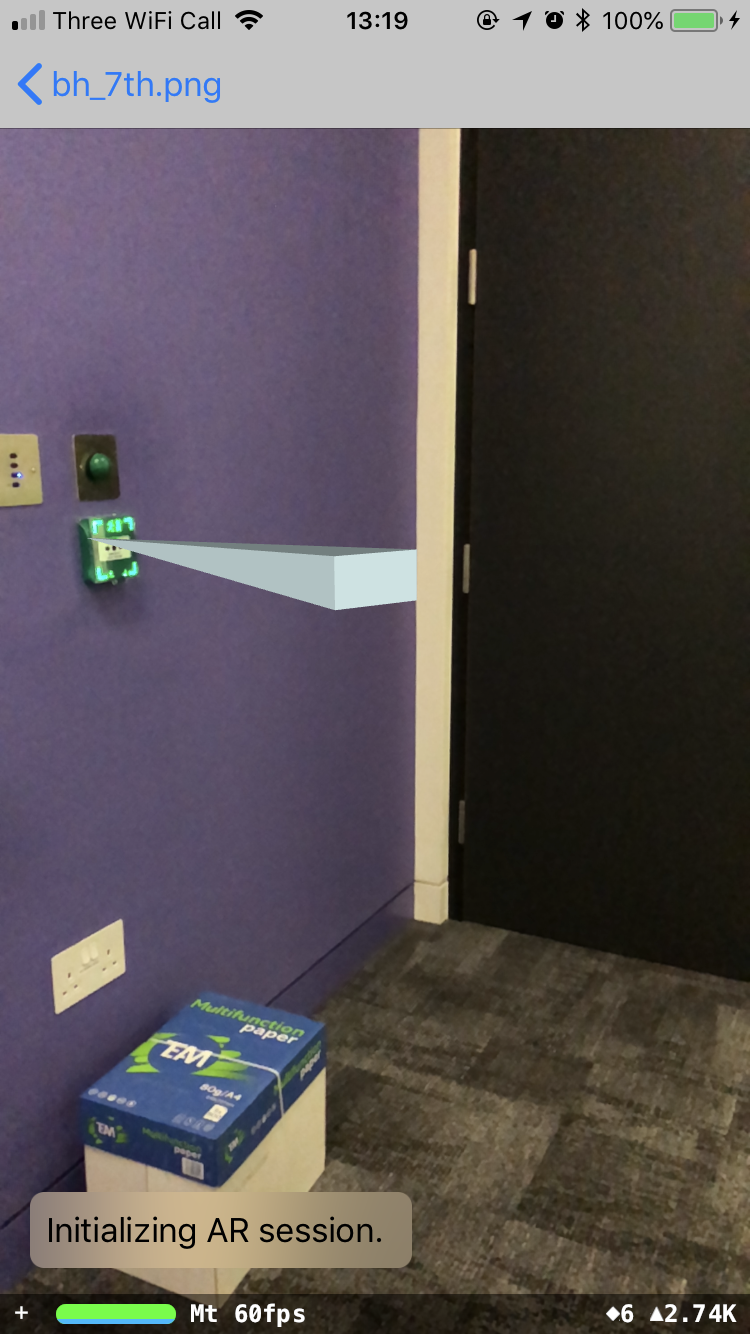
\includegraphics[width=180px, height=320px]{Evaluation/AR-arrow.png}
    \caption{Screen shot taken from the user mobile app which shows the guidance arrow for navigation}
    \label{fig:ar-arrow}
\end{figure}

\newpage
Additionally, the app is able to pull information from the King's services in order to show timetable information and computer availability. However, at present, the computer availability feature is a proof of concept, showing the same data for each room. This is because PC-Free@King's has information for only one room in Bush House, 4.02.

\begin{figure}[H]
    \centering
    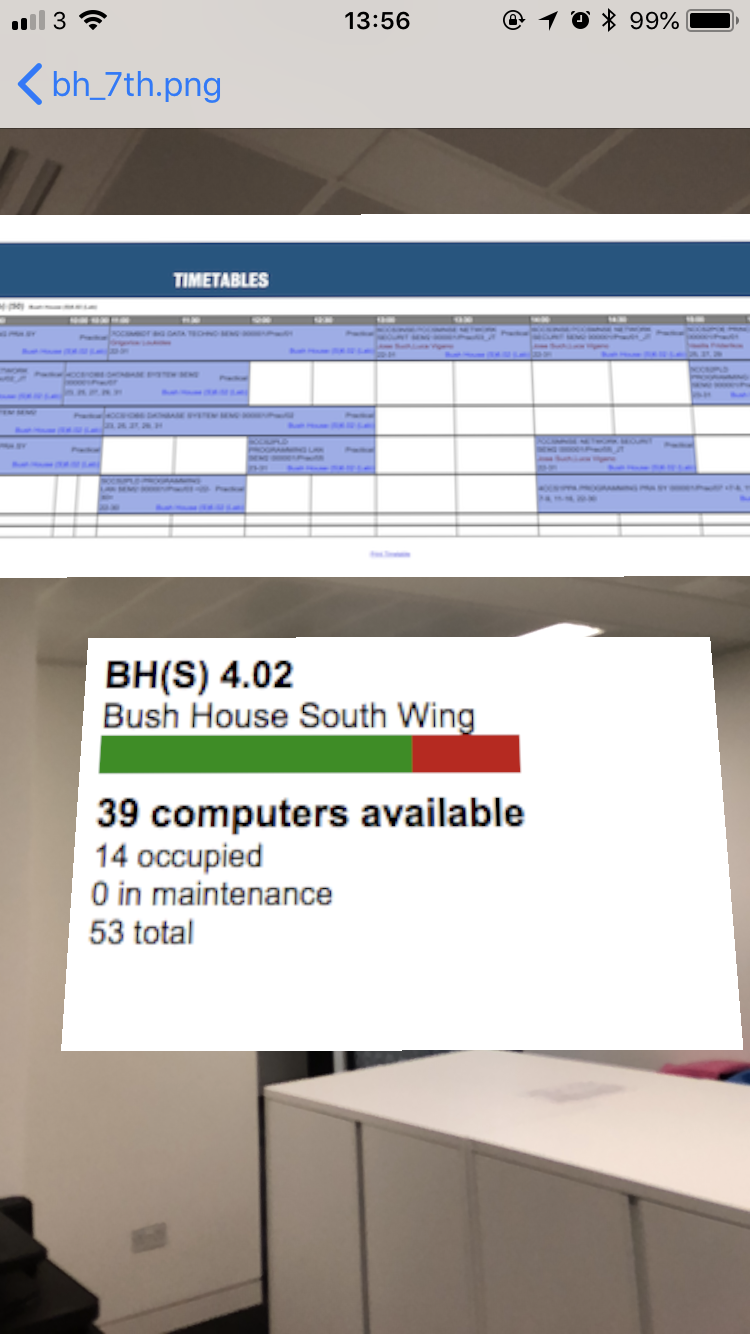
\includegraphics[width=180px, height=320px]{Evaluation/AR-Info.png}
    \caption{Screen shot taken from the user mobile app which shows the information displayed.}
    \label{fig:ar-info}
\end{figure}

\section{Project Evaluation}

\subsection{Functional Evaluation}
The project is able to scan and save Wi-Fi measurements, use them to position a user, and then provide navigation instructions for users to find their way around Bush House. All the requirements set out in chapter 4 were completed and fully tested. An empirical evaluation of the project that looks at how accurate the system is has been provided in sections \ref{sec:accuracy}, \ref{sec:nav-analysis}, and \ref{sec:ar-results}. In order to evaluate the key requirements necessary to meet the project aims, a non-functional evaluation, focused more on quality attributes, will be further detailed in the next section.

\subsection{Non-functional Evaluation}
\begin{itemize}
    \item Requirement: \textit{Interoperability – The subsystems should be able to fully integrate with other subsystems in order to provide maximum flexibility.} (section \ref{sec:non-functional-reqs}
    
    As mentioned in the design and in the implementation chapters, all the servers and data providers have an API to communicate with other components of the system. The data management server has a RESTful API to access the database, the Positioning \& Path Finder system has an API in order to calculate data and provide results, and the AR Data Provider has an API that provides required data to show in the user application. All the communications that take place using the APIs use a JSON format, which is a very popular serialisation format. In this way interoperability has been achieved, by integrating all the systems through the REST APIs which communicate using the JSON format.
    
    \item Requirement: \textit{Maintainability – The system should provide a simple and easy way to extend feature base. For this, the follow concepts must be followed}:
        \begin{itemize}
            \item Sub-requirement: \textit{Separation of Systems – The system must be decomposed in multiple independent subsystems which must be as decoupled as possible. The systems should use the appropriate programming languages and framework to achieve their requirements and tasks.}
            \newline\newline
            The architecture components have been separated first into layers that achieve common goals, and then into separate systems, depending on the task achieved. The user mobile application and admin mobile application have been separated due to the nature of the features, and then based on the data that each handles, the other systems have been decoupled. This is detailed extensively in the design chapter. Because systems are very separated, any of them can be easily replaced without affecting the system as a whole. For example, mobile applications could be developed for other operating systems, such as Android.
            \item Sub-requirement: \textit{Architectural Patterns – Each subsystem should follow the appropriate architectural pattern and design patterns provided by the framework that is being used, or the programming language that the system is written in.}
            \newline\newline
            The best practices and design patterns have been used when appropriate, in each application. Most of the system makes use of an MVC design pattern, mainly due to the frameworks that they use, and the way those have been designed. Evidence of the MVC pattern is presented in the design chapter, along with the code listed in the implementation chapter and the appendix.
        \end{itemize}
        Overall, the separation of systems and the architectural patterns have been considered so that the system is maintainable.
    \item Requirement: \textit{Usability – The system should provide an easy to use interface, and as clear as possible. Although it can be simple, the interfaces must provide clarity of interactions, and a satisfactory user experience.}
    \newline\newline
    The GUI of the mobile applications has been made clear and simple, by incorporating system visual elements. These elements are used across iOS, therefore, the user is familiar with the way they should interact. For long waiting times in the apps, spinners have been used to keep let the user know that data is loaded, and the application is still running. The floor plan images have been fitted to all screen sizes, and a search bar was used to make it easier to look for rooms.  
\end{itemize}

% \subsection{Limitations}

% In results, talk about the overhead that the HTTP request bring for example to the positioning algorithm, or even the navigation algorithm.

\section{Comparison to other existing solutions}
\label{sec:comparison}
When comparing the navigation system built in this project to other existing solutions, the most suitable comparison would be with "Indoor Survey App" \cite{apple-indoor-survey}. The app built by Apple is the most relevant, as the data is measured using the same technique, but this project's solution provides an arguably better and more extensible system. Below, a full comparison is detailed.

The most important comparison that can be made with Apple's solution is the architecture of the system. A very important aspect to remember is that Indoor Survey App provides positioning and measuring for any building that follows their specific requirements, whereas the app in this project only supports Bush House. However, this is a feature that can be easily added on top of the existing capabilities, since the system has been developed with extensibility in mind.

The way that both of the apps measure relevant positions in the buildings is by using the floor plans. After the user registers their floor plans and has them available in the app, they can record important reference points in the building by tapping on the screen. This will register the position on the image and assign Wi-Fi measurements to it. Even though the ways of working are more or less the same, the system created in this project can support any measuring platform, for an example Android device, whereas Apple's will only run on iOS. However, performance-wise, Apple's application is faster when dealing with scanning for Wi-Fi networks, because all the measurements take place on the phone, and not through a multitude of systems. Nevertheless, if the scanning module that is available on the mobile device would be made open by Apple, this can be easily adopted by our application without any difficulties. This will be detailed in the limitations and future work chapter.

Furthermore, Apple's application is limited to buildings and venues that "attract more than one million visitors annually" \cite{apple-indoor-survey}. Although the system only supports Bush House, as future work, it can be easily extended to any building that has its floor plans available, with no limit on the number of visitors. It is not clear right now, due to user restriction, if Apple's application supports anything more than just measuring buildings and then positioning users, but our system comes at an advantage because this project's solution uses navigation and also makes use of AR features by using ARKit to improve the user's experience.

Another solution that has a fingerprinting based approach is SLAM \cite{SLAM}. SLAM tries to improve this approach by eliminating the offline measuring process, which brings a lot of limitations by the fact that the area must be surveyed before using the positioning system. This solution brings tracking on unknown grounds and does not have to record data in advance, such as the floor plan; nonetheless, if available, a data set can be connected and used. However, this type of approach comes with a drawback that is very important if implemented on mobile devices: a very high computational load. This makes it unfeasible to use on mobile devices, because of the limited resources available and because the energy use would be significant. In this case, even though our approach requires the admin user to make prior measurements of the floor plans, the energy use is very low, because all the calculations are being made on an external server.
